\documentclass{article}
\usepackage[paperheight=5in,paperwidth=11in,margin=.2in]{geometry}
\usepackage[sfdefault]{roboto}
\usepackage[T1]{fontenc}
\usepackage{graphicx}

\begin{document}
\pagenumbering{gobble}
\begin{samepage}

\noindent \textbf{Supplemental Figure S1.}
Positions supported by short Illumina reads in the telomeric candidate long-read sequences on \textbf{(A)} \textit{p} arms and \textbf{(B)} \textit{q} arms of datasets HG001 through HG007 (sequences from all datasets are plotted together).
Long reads are plotted in blue, and positions supported by short reads are marked in green.
Genomic coordinates are given in kbp, relative to the boundary of the annotated telomeric tract.
Note that, due to the multi-kbp scale, individual small supported/unsupported regions may not be visible.

\begin{figure}[h!] \centering
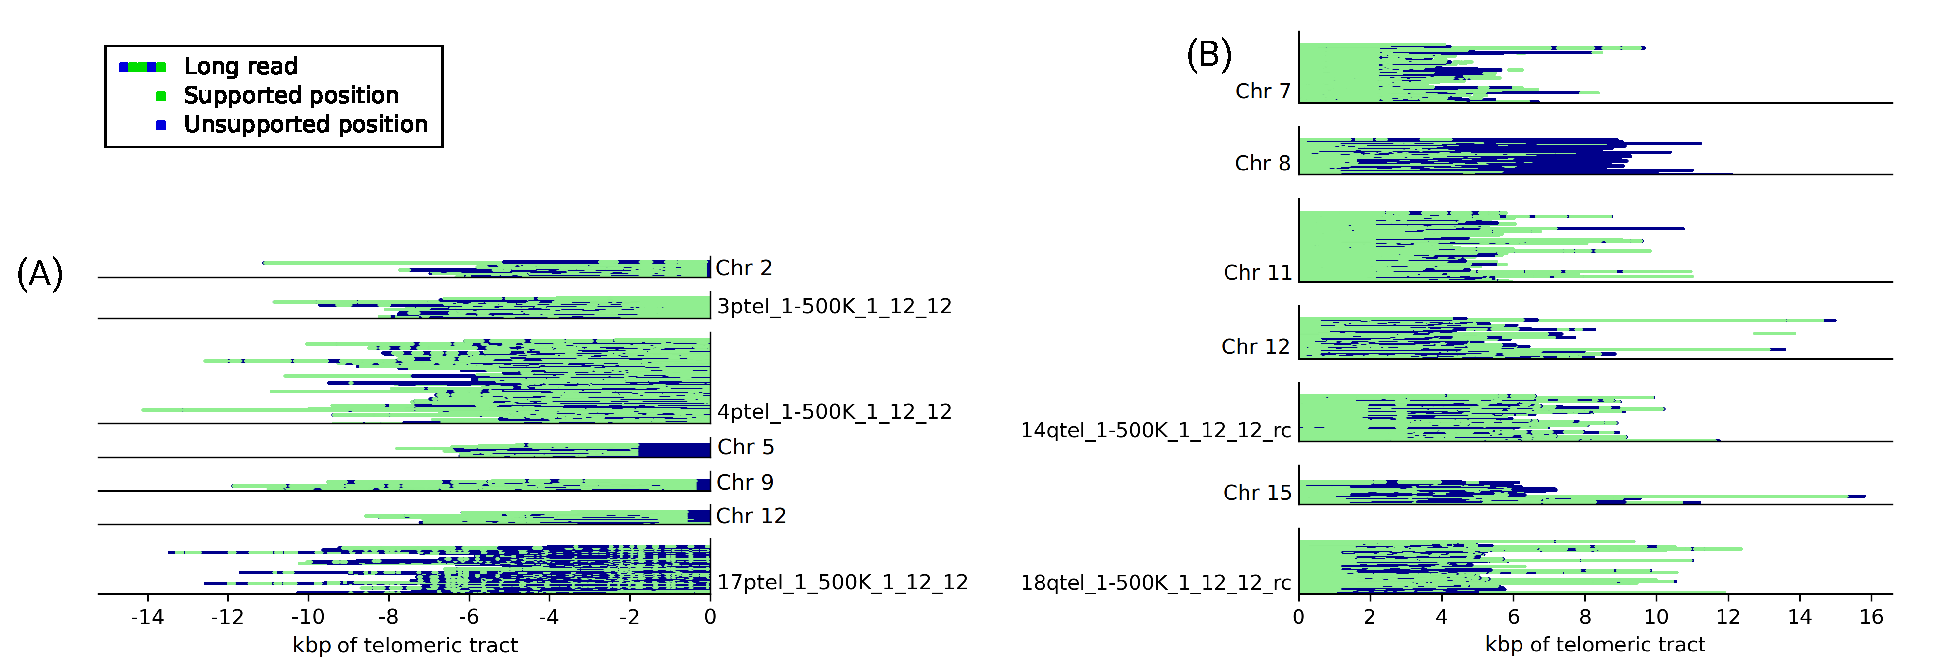
\includegraphics[width=\textwidth,keepaspectratio]{Figure_S1-nolegend.pdf}
\end{figure}

\end{samepage}
\end{document}
